\documentclass[conference]{IEEEtran}
\IEEEoverridecommandlockouts
% The preceding line is only needed to identify funding in the first footnote. If that is unneeded, please comment it out.
\usepackage{cite}
\usepackage{amsmath,amssymb,amsfonts}
\usepackage{algorithmic}
\usepackage{graphicx}
\usepackage{textcomp}
\usepackage{xcolor}
\def\BibTeX{{\rm B\kern-.05em{\sc i\kern-.025em b}\kern-.08em
    T\kern-.1667em\lower.7ex\hbox{E}\kern-.125emX}}
\begin{document}

\title{Experimental investigation of forced convective heat transfer in cylindrical pipe flow\\
%{\footnotesize \textsuperscript{*}Note: Sub-titles are not captured in Xplore and should not be used}
%\thanks{Identify applicable funding agency here. If none, delete this.}
}

\author{\IEEEauthorblockN{Yoshinori Hattori}
\IEEEauthorblockA{\textit{Shibaura Institute of Technology, Mechanical Engineering}\\
Tokyo, Japan \\
%\textit{Graz University of Technology, Institute of Fluid Mechanics and Heat Transfer}\\
%Graz, Austria \\
md18060@shibaura-it.ac.jp}}

\maketitle

%\begin{abstract}
%This document is a model and instructions for \LaTeX.
%This and the IEEEtran.cls file define the components of your paper [title, text, heads, etc.]. *CRITICAL: Do Not Use Symbols, Special Characters, Footnotes,
%or Math in Paper Title or Abstract.
%\end{abstract}

\begin{IEEEkeywords}
Forced convection, Nusselt number, Wall friction, transitional, Cylindrical pipe flow
\end{IEEEkeywords}

\section{Introduction}
Forced convective heat transfer in cylindrical pipe flow plays an important role in many technical cooling systems.
These coolant technology is used wide varaety of coolant applications such as electric devices, automotive, and plant factory.
Considering heat transfer issues, heat transfer coefficient is one of the most important numbers.

Much remains to be studied for providing experimental data for high Pramdlt number and laminar-to-turbulent transitional regime.
In this paper, we focus on forced convective heat transfer in cylindrical pipe flow in particular high Pramdlt number and transitional regime.
%The experiment was carried out considering a board range of Reynolds number, spanning from laminar to fully turbulent flow.
A 50/50vol\% mixture of water and glycole which is a typical liquid coolant in automotive applications were used as a operating fluid.
This coolant liquid is normally used in low temperature.
However, it's difficult to maintain the cylindical pipe at low temperature.
Therefore, as a 1st approach, we take a data for high temperature and then compared with Direct Numerical Simulation (DNS).
If there is a good agreement between experimental data for high temperature and DNS, the result in a low temperature would be predicted by DNS.
%In this paper we apply the techniques of Laser-induced fluorescence (LIF) to find out temperature distribution in cylindrical pipe flow.
Moreover, the investigation shall also include the measurement of wall friction coefficient.
The engineeres is frequently interested in pressure drop which is related to determine pump or fan power equipments.
%The experimental data compared with some correlations and other sources as well as computational results obtained from already existing numerical simulations (CFD) by Rorenzo\cite{Rorenzo2019}.

%\section{The phenomena}
%%Temperature variations for constantHeat flux
%\begin{figure}[htbp]
%  \centering
%  %\vspace{-3zh}
%  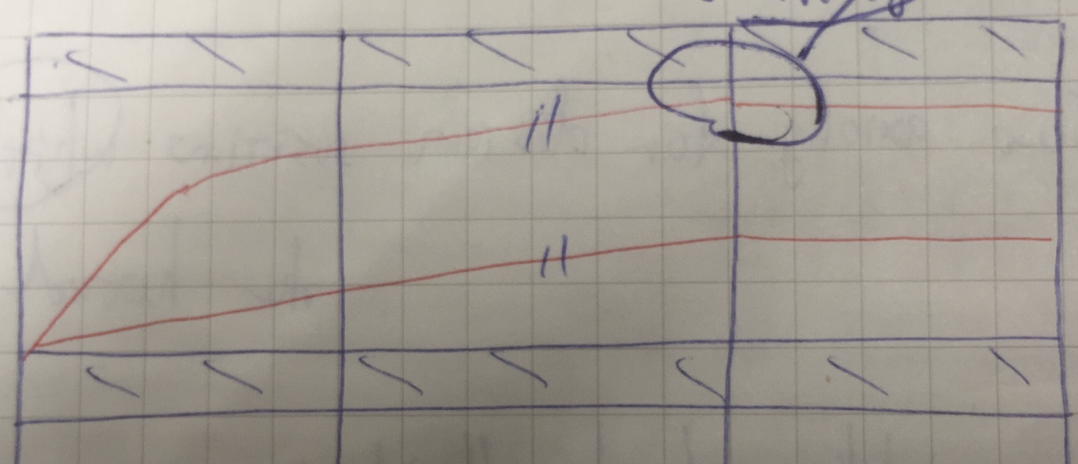
\includegraphics[width=0.47\textwidth,natwidth=610,natheight=642]{fig/temperature_variations_constant_heat_flux.png}
%  \caption{Temperature variations for constantHeat flux}
%  \label{temperature_variations_constant_heat_flux}
%\end{figure}
%
%%Heat transfer coefficient depend on x value
%Figure\label{heat_transfer_coefficient_depend_on_x_value} shows the local heat transfer coeeficient 
%\begin{figure}[htbp]
%  \centering
%  %\vspace{-3zh}
%  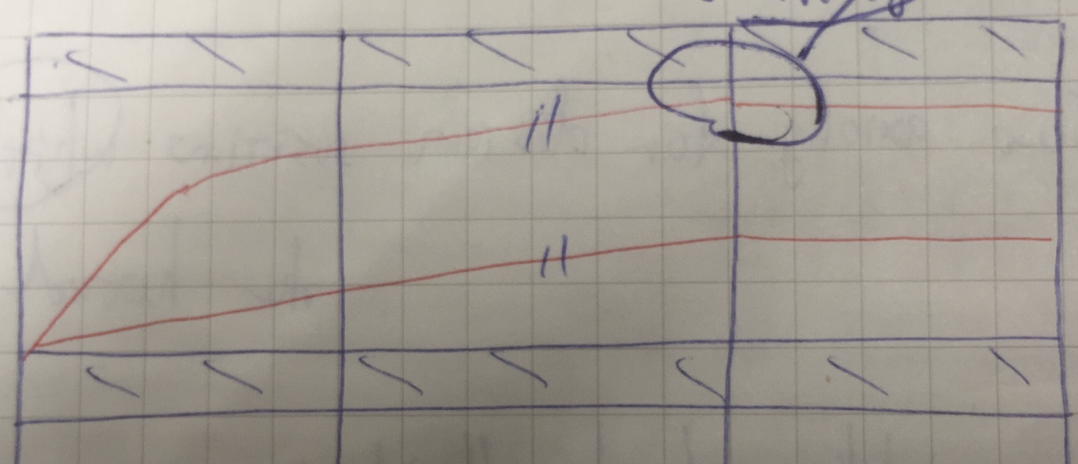
\includegraphics[width=0.47\textwidth,natwidth=610,natheight=642]{fig/temperature_variations_constant_heat_flux.png}
%  \caption{Heat transfer coefficient depend on x value}
%  \label{heat_transfer_coefficient_depend_on_x_value}
%\end{figure}
%There are two surface conditions arise in many engineering applications.
%One is constant surface heat flux and the other is constant surface temperature.
%In the fully developed flow of the tube, fluid constant porperties, the local heat coefficient is constant independent of x.

\section{The phenomena}
%Experimental Setup
Figure\label{experimental_loop} shows experimental setup which is already existing facilities by Christphan\cite{Christphan2018}.
\begin{figure}[htbp]
  \centering
  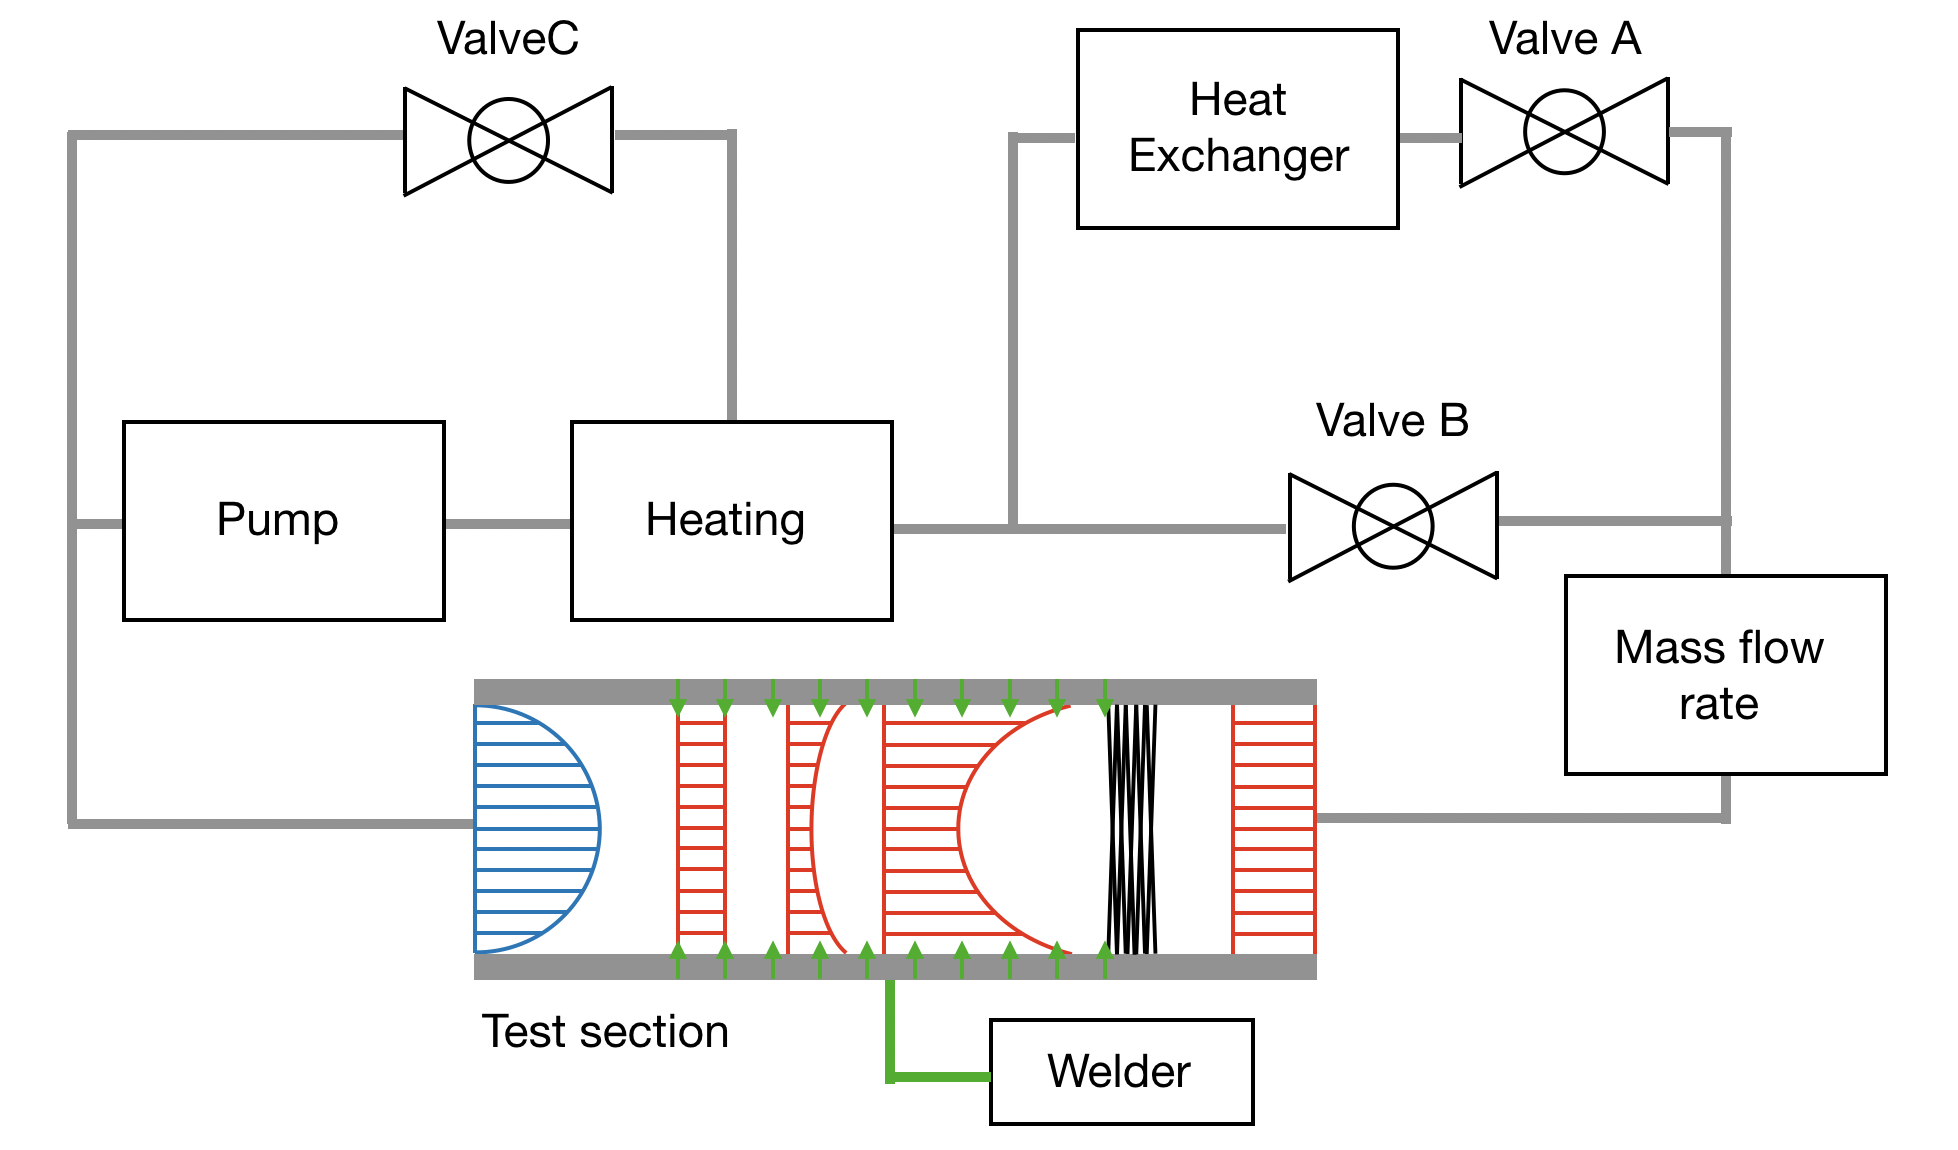
\includegraphics[width=0.47\textwidth,natwidth=920,natheight=700]{fig/experimental_loop.png}
  \caption{Experimental loop.}
  \label{experimental_loop}
  \vspace{-2zh}
\end{figure}
The experimental loop consists of heat exchanger, pump, coriolis mass flow rate, welder, reservoir, and test section basically.
Heat exchenger keep thermal stationary condition in flow pipe.
Mass flow rate is controlled by pump and baypass valve C which is located in a parallel.
The pipe is thermal isolated, surrounded with glass wool.\\

Figure\label{thermal_boundary_layer_development} shows velocity and thermal boundary layer development vary with horizontal axis in a test section.
Velocity and thermal profile are shown blue and red color, respectively.
The test section is made of stainless steel (1.4301) with an inner diameter di=12mm and outer diameter do= 15mm.
Highly accurate resistance thermall probes (PT-100) are used to find out the inlet and outlet bulk temperature (Tib , Tob) and wall temperature Tw.
Moreover, thermocouple 'Type-K' are used to take temperature gradient in flow direction.
(See ''science problems and interesting issue'' section No.3.)
However, those thermocouples aren't directly related to calculete four parameters. (Re, Nu, Pr, Cf)
The test section consist of entrance, heated and thermal equalized part.
\begin{enumerate}
  \item Entrance part\\
  The first part of test section is 1.2[m] length entrance part which is sufficiently long to ensure dynamically developed flow condition at the exist.
  (See ''science problems and interesting issue'' section No.4.)
  The bulk temperature (Tb0) at this section were measured by PT-100.
  \item Heated part\\
  The second part of test section is 2[m] length heated part which is sufficiently long to ensure thermaly fully developed flow condition at the exist.
  The tube wall were heated electrically by welder which provide high current and low voltage to keep the uniform heat flux condition in a inner pipe flow. 
  Convective heat transfer is independent with horizontal axis in fully developed flow, constant heat flux condition.
  The wall temperature (Tw) at the exist of this section were measured by PT-100.
  \item Thermal equalized part\\
  The third part of test section is thermall equalized part which is including static mixture. Static mixture forms turbulent and vortex. Then, the thermal profile of heated exist mix together. At the end, the bulk temperature(Tb1) are measured.
\end{enumerate}


\begin{figure}[htbp]
  \centering
  %\vspace{-3zh}
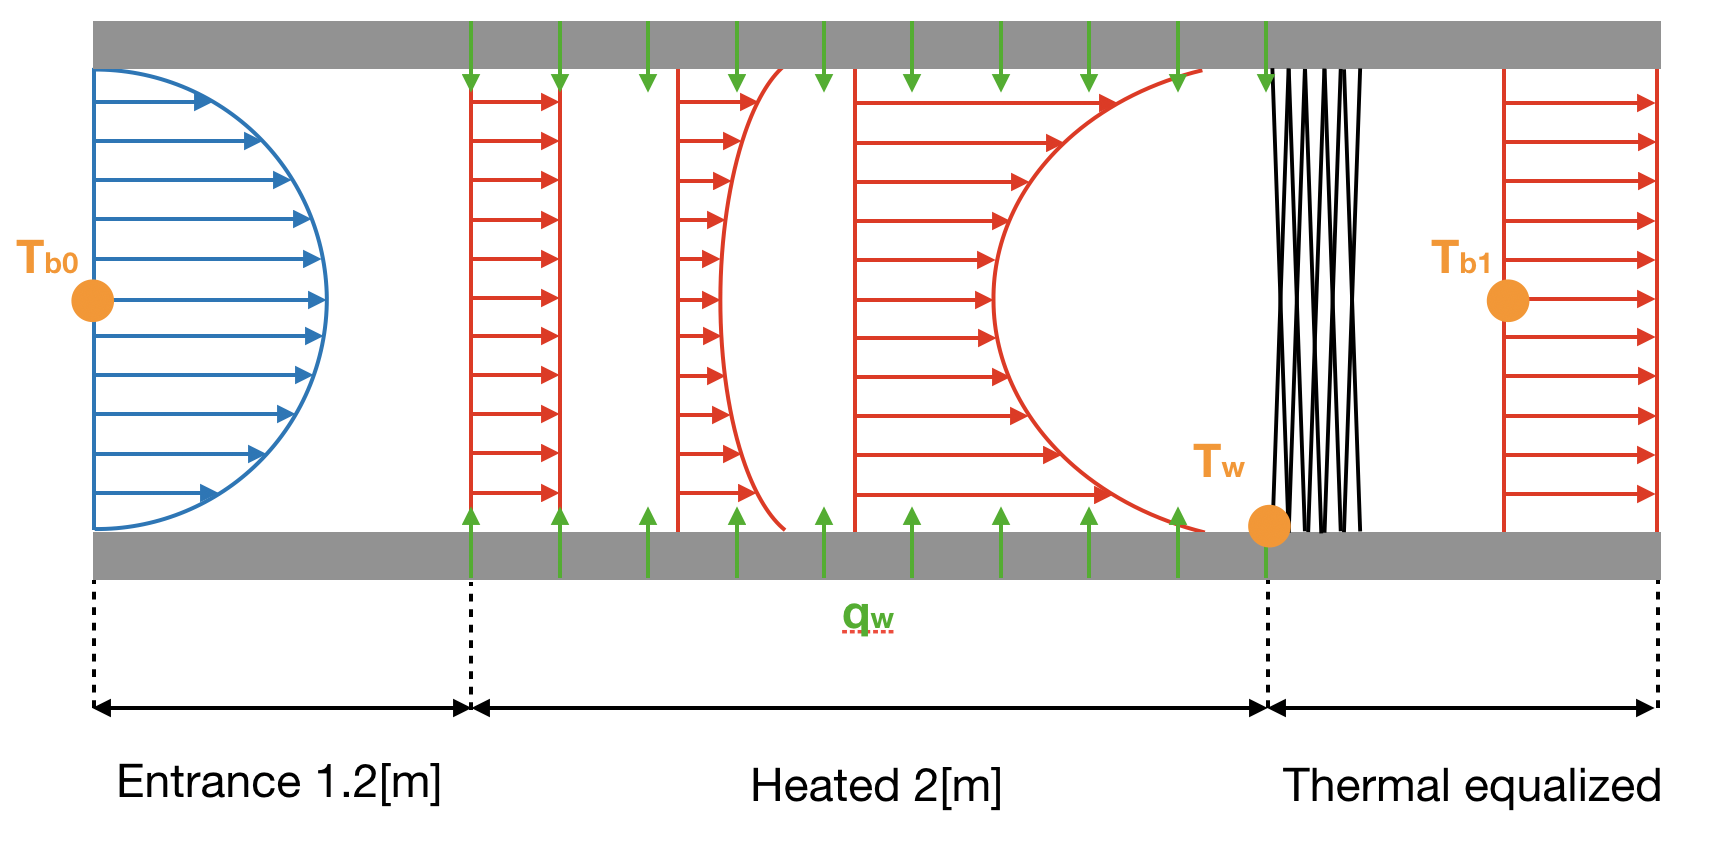
\includegraphics[width=0.47\textwidth,natwidth=850,natheight=450]{fig/thermal_boundary_layer_development.png}
  \caption{Velocity (blue) and thermal (red) boundary layer development vary with horizontal axis in a test section.}
  \label{thermal_boundary_layer_development}
\end{figure}

There are 3 ways to control Re and Pr, the value which we need.
It is hard to keep high Pr and low Re.
Figure 3-8 shows material properties of Shell Heat Transfer Oil S2.

\begin{enumerate}
  \item Cooling water\\
  As opening valve A and closing valve B, decreasing flow temperature.
  Then, viscosity increase and Re decrease and Pr increase.
  \item Bypass pipe\\
  As opening bypass pipe C, decreasing mass flow rate then, Re decrease.
  As decreasing mass flow rate, Pr decrease because the number is related to heat transfer convection from the wall. ( Heat is provided from the wall.)
  In order to decrease mass flow rate, controlling bypass pipe is stronger than pump machine.
  \item Welder and mass pump machine\\
  As decreasing mass flow rate (pump machine) and welder, Re decrease and Pr is kept nearly constant.
  Pr is proposonal to Nu which is, convection devided by conduction.
  Controlling both welder and mass flow rate, the ratio is maintained constant value.
\end{enumerate}
Those method are in a unquantative way.
(See ''science problems and interesting issue'' section No.1.2.)

\begin{figure}[h]
\vspace{3zh}
\begin{minipage}{0.48\linewidth}
 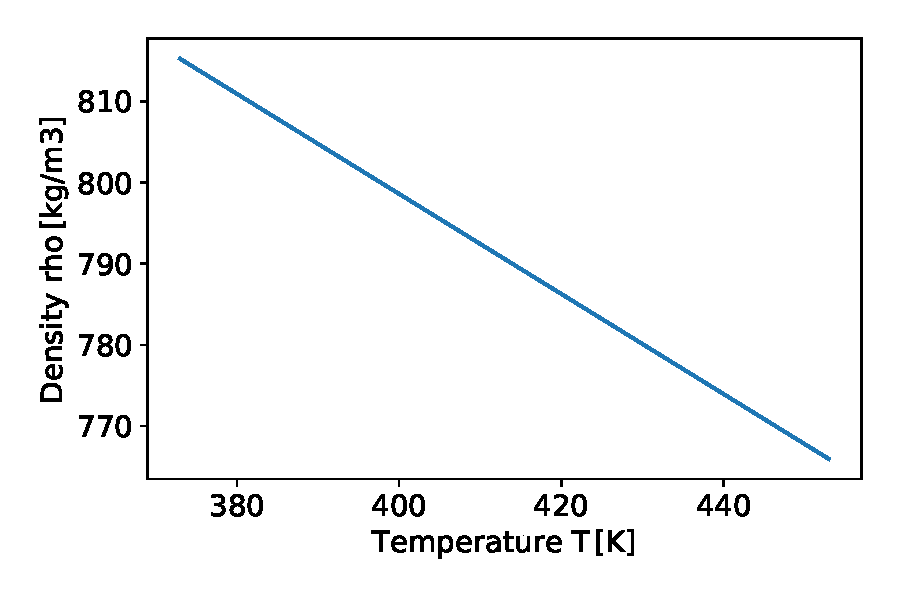
\includegraphics[width=0.48\textwidth,natwidth=200,natheight=220]{fig/density_rho.pdf}
 \vspace{-1.5zh}
 \caption{Density rho, $\rm kg/m^{3}$}\label{density_rho}
\end{minipage}
\hfill
\begin{minipage}{0.48\linewidth}
 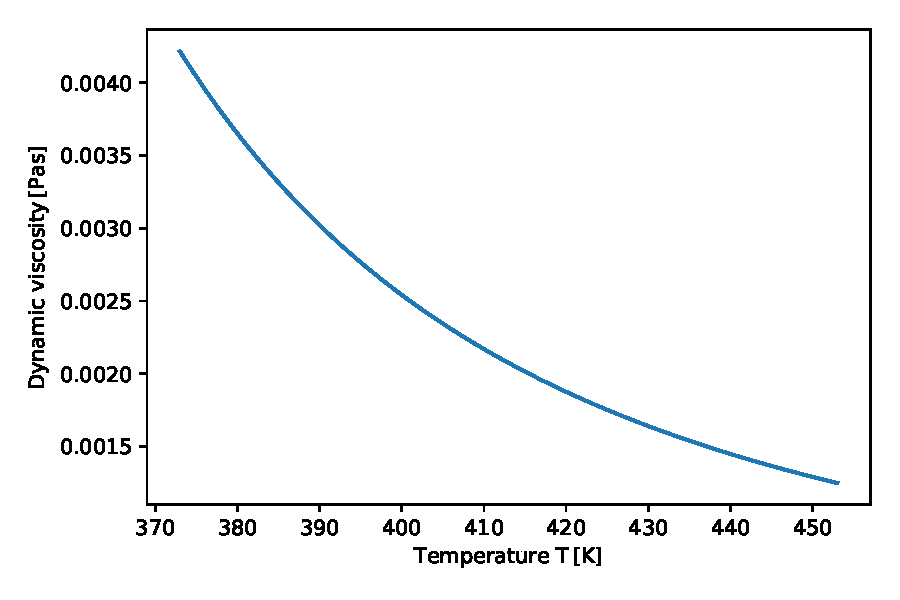
\includegraphics[width=0.48\textwidth,natwidth=190,natheight=210]{fig/dynamic_viscosity.pdf}
 \vspace{-1.5zh}
 \caption{Dynamic viscosity mu, $\rm Pa s$}\label{dynamic_viscosity}
\end{minipage}
\vspace{2zh}
\end{figure}

\begin{figure}[h]
\vspace{1zh}
\begin{minipage}{0.48\linewidth}
 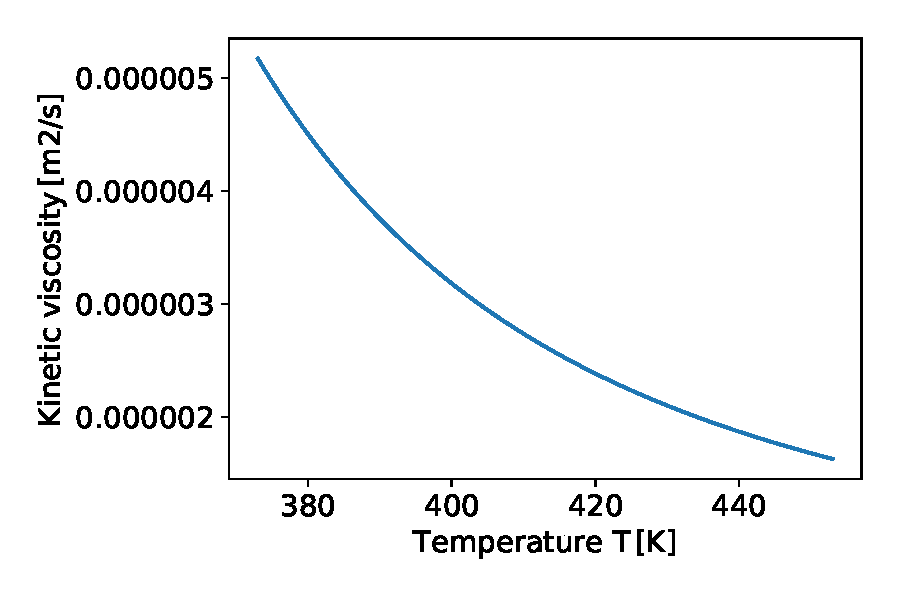
\includegraphics[width=0.48\textwidth,natwidth=200,natheight=220]{fig/kinetic_viscosity.pdf}
 \vspace{-1zh}
 \caption{Kinetic viscosity nu, $\rm m^{2}/s$}\label{kinetic_viscosity}
\end{minipage}
\hfill
\begin{minipage}{0.48\linewidth}
 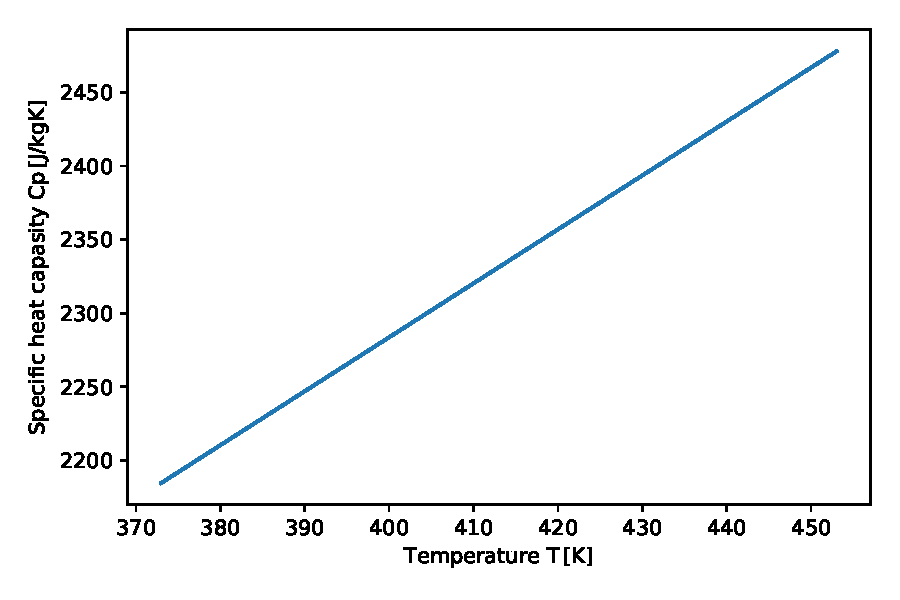
\includegraphics[width=0.48\textwidth,natwidth=190,natheight=210]{fig/heat_capacity.pdf}
 \vspace{-1.5zh}
 \caption{Heat capacity Cp, $\rm J/kgK$}\label{heat_capacity}
\end{minipage}
\vspace{2zh}
\end{figure}

\begin{figure}[h]
%\vspace{-1.5zh}
\begin{minipage}{0.48\linewidth}
 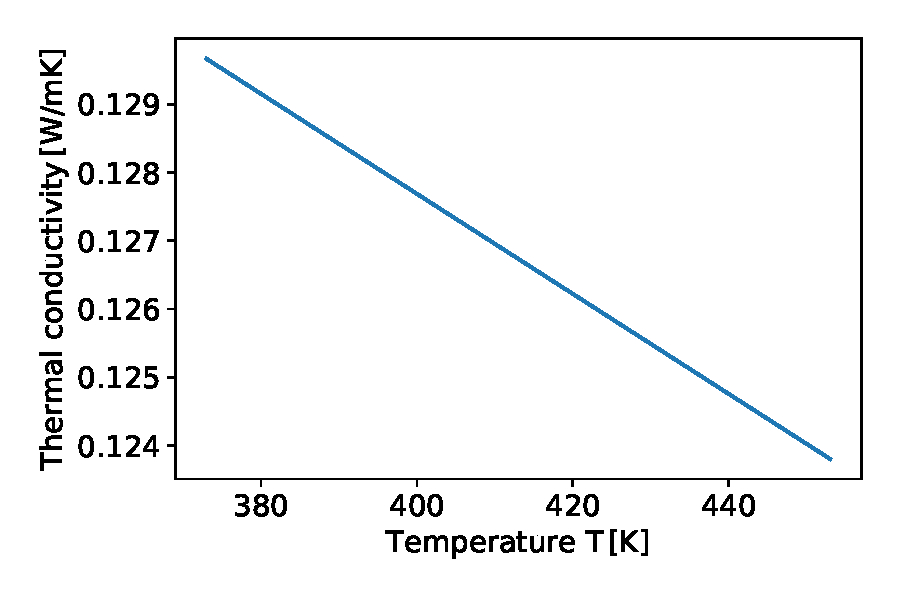
\includegraphics[width=0.48\textwidth,natwidth=190,natheight=210]{fig/thermal_conductivity.pdf}
 \vspace{-1.5zh}
 \caption{Thermal conductivity, $\rm W / m k$}\label{thermal_conductivity}
\end{minipage}
\hfill
\begin{minipage}{0.48\linewidth}
 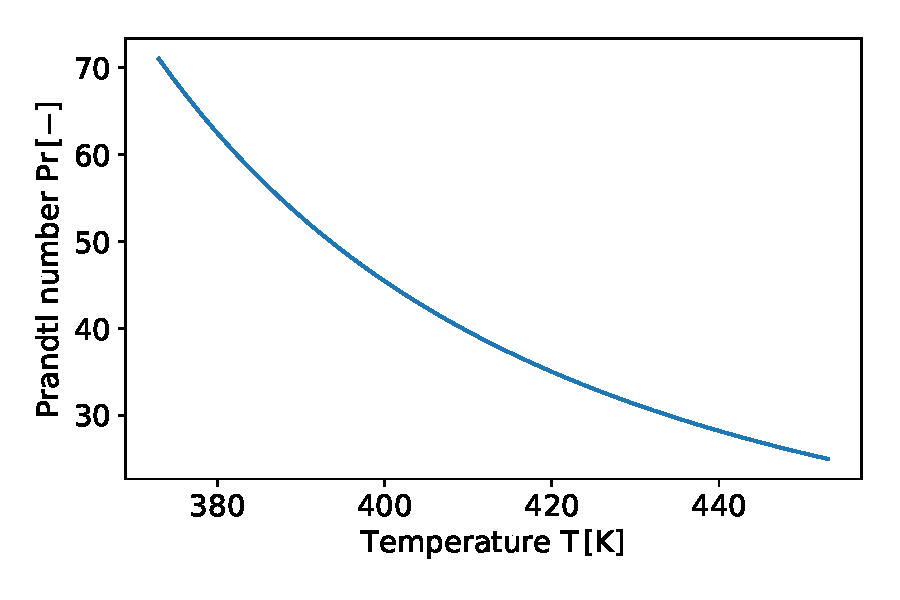
\includegraphics[width=0.48\textwidth,natwidth=190,natheight=210]{fig/prandtl_number.pdf}
 \vspace{-1.5zh}
 \caption{Prandtl number Pr, -}\label{prandtl_number}
\end{minipage}
%\vspace{-2zh}
\end{figure}

%\begin{figure}[h]
% \begin{minipage}{0.48\linewidth}
% \begin{center}
%   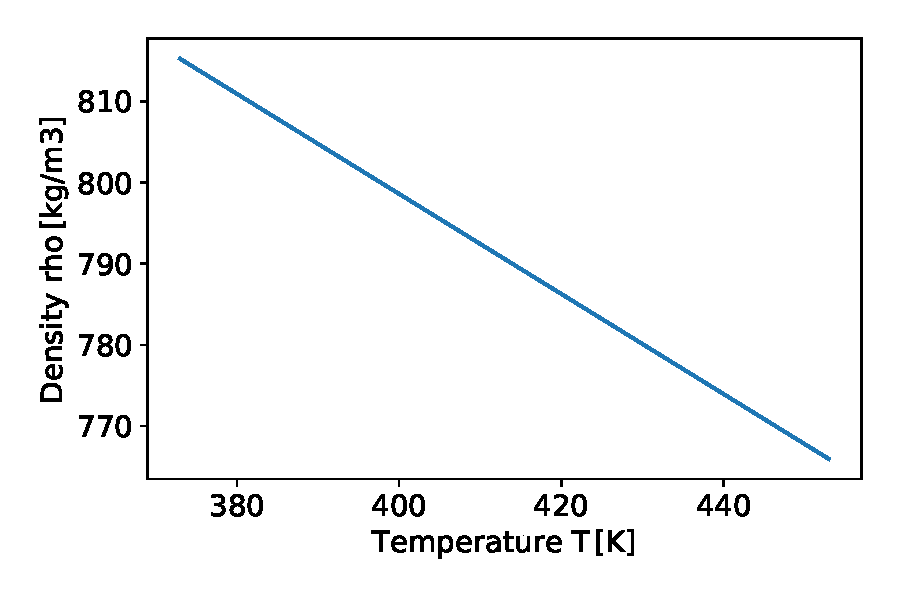
\includegraphics[width=0.47\textwidth,natwidth=280,natheight=300]{fig/density_rho.pdf}
%  \end{center}
%  \caption{$q=50\,\rm kW/m^2$ \cite{Inoue2016}}\label{HeatFlux=50k}
% \end{minipage}
% \hfill
% \begin{minipage}{0.48\linewidth}
% \begin{center}
%   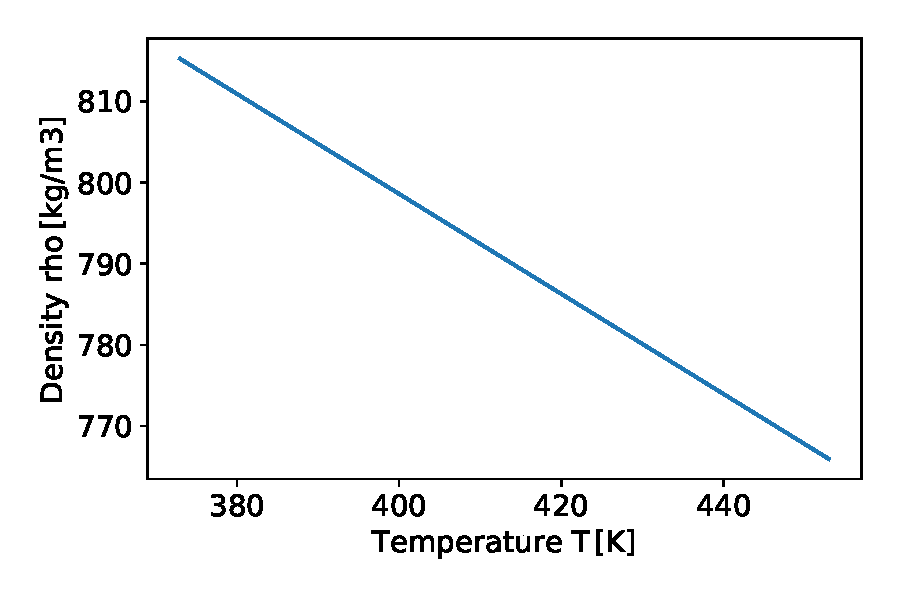
\includegraphics[width=0.47\textwidth,natwidth=610,natheight=642]{fig/density_rho.pdf}
%  \end{center}
%  \caption{$q=50\,\rm kW/m^2$ \cite{Inoue2016}}\label{HeatFlux=50k}
% \end{minipage}
% \vspace{-2zh}
%\end{figure}

\newpage
\section{Calucuration Flow}
Material properties are temperature-dependent function.
At first, material properties vary with temperature are taken.
Next, we move to experimental facilities and measure temperature difference, pressure difference and mass flow rate.
Finaly, Nusselt, Prandtl, Reynolds numbers and friction coefficient are calcurated by post-proccesing, MATLAB. 
In order to disscuss the issue, experimental data are compared with next correlations.

\section{Correlations}
Skinf friction coefficient for laminar flow is descrived following equation.
\begin{equation}
C_{f,lam}=\frac{16}{Re_{b}}
\end{equation}
Konakov\cite{Konakov1954} showed skin friction coefficient for turbulent flow.
\begin{equation}
C_{f,turb}=0.25(1.8log(Re_{b})-1.5)^{-2}
\end{equation}
Note that these skin friction coefficient just suitable for no-heating condition, constant fluid properties.
In this thesis, we provide heat to the pipe.
Therefore, the fluid properties change depend on the temperature.

From general dimensional analysis, Nusselt number represents function of Reynolds number (Re) times Prandtl number (Pr) as following equation.
\begin{equation}
Nu=\alpha \cdot Re^{\pi_{\beta}}\cdot Pr^{\pi_{\gamma}}\label{Nu_dimensional}
\end{equation}
Here, factors $\alpha$, $\beta$ and $\gamma$ are constant value depend on flow regime and calcurated from numerical experimental results.
Gunienski\cite{Gnienlinski2010} showed correlations for each flow regime laminar and turbulent, respectively.
Gunienski\cite{Gnienlinski2010} showed calculation method for laminar flow.
\begin{equation}
Nu_{lam}=(3.66^{3}+0.7^{3}+(1.615(Re_{b}Pr_{b}\frac{d_{i}}{L})^{1/3})^{3})^{1/3}\label{Nu_laminar}
\end{equation}
%The range 0.1<<Pr_{b}<<1000, 10^{4}<<Re_{b}<<10^{6}.
Gunienski\cite{Gnienlinski2010} showed calculation method for turbulent flow.
\begin{equation}
Nu_{turb}=\frac{\frac{C_{f}}{2Re\cdot Pr_{b}}}{1+12.7 \sqrt{\frac{C_{f}}{2}}(Pr_{b}^{2/3}-1)}\cdot (\frac{Pr_{b}}{Pr_{w}})^{0.11}
%Nu_{turb}=\frac{\frac{C_{f}}{2\cdot Re\cdot Pr_{b}}{(1+12.7\frac{C_{f}}{2}}\cdot (Pr^{\frac{2}{3}}-1)}\cdot(1+(\frac{d_{h}}{l})^{\frac{2}{3}})\label{Nu_turblent}
\end{equation}
The range is
\begin{equation}
0.1<<Pr_{b}<<1000, 10^{4}<<Re_{b}<<10^{6}.
\end{equation}
He presented transitional flow as a liner interpolation between turbulent and laminar flow.
(See ''science problems and interesting issue'' section No.12.)
\begin{equation}
Nu_{m}=(1-r)Nu_{m,lam}+rNu_{m,turb}
\label{Nu_m}
\end{equation}
\begin{equation}
r=\frac{Re_{b}-2300}{10^{4}-2300}
\end{equation}
\\

\section{State-of-the-art}
The presentaly considerd oil is Shell Heat Transfer oil S2.
The result show good agreement with correlations.
We are going to use water-glycole as a operationg liquid.\\

\section{Scientific problems and interests issues}
\begin{enumerate}
  \item Quantative way\\
  There are 3 valves, A, B and C in the experimental loop.
  The experimental condition Re and Pr are controlled by those 3 valves, pump and welder.
  The pump and welder can control in a quantative way.
  However, those 3 valves are controlled by human hand and those are no certain value.
  In this report, that's the reason why I just say INCEASE or DECREADE, unquantative way.
  Therefore, to controlle 3 valves in a quantative way are needed.\\
  \item Fluid properties\\
  Density, heat conductivity, specific heat transfer Cp, nu, mu, Pr are all varies with temperature shown as temperature dependance in figures 3-8. of fluid properties.
  It is difficult to reach high Pramdlt number and transitional Reynolds number, which we really want.
  For example, as enhance cooling, temperature decrease, statics viscosity increase.
  As a result, Pr increase and Re decrease.
  There are 3 ways to controlle Pr and Re shown in ''Experimental loop and Method'' section.
  Pr and Re are related each other and it it difficult to maintain the value that we want to measure.
  This problem is related mere close to ''quantative way'' shown above.
  Therefore, we need to find solution which is able to reach the value in an optimal way, not rule-of-thumb.\\
  \item Temperature calibration\\
  There are two kinds of temperature measurement, PT-100 and thermocouples.
  Thermocouples are calibrated by PT-100 because PT-100 is more accurate than thermocouples.
  Here, there is a interesting issue.
  When we calibrate, thermocouples temperature of initial condition are always lower than PT-100.
  Figure.9 shows monitored thermocouples and PT-100 before calibration.
\begin{figure}[h]
\vspace{3zh}
  \centering
  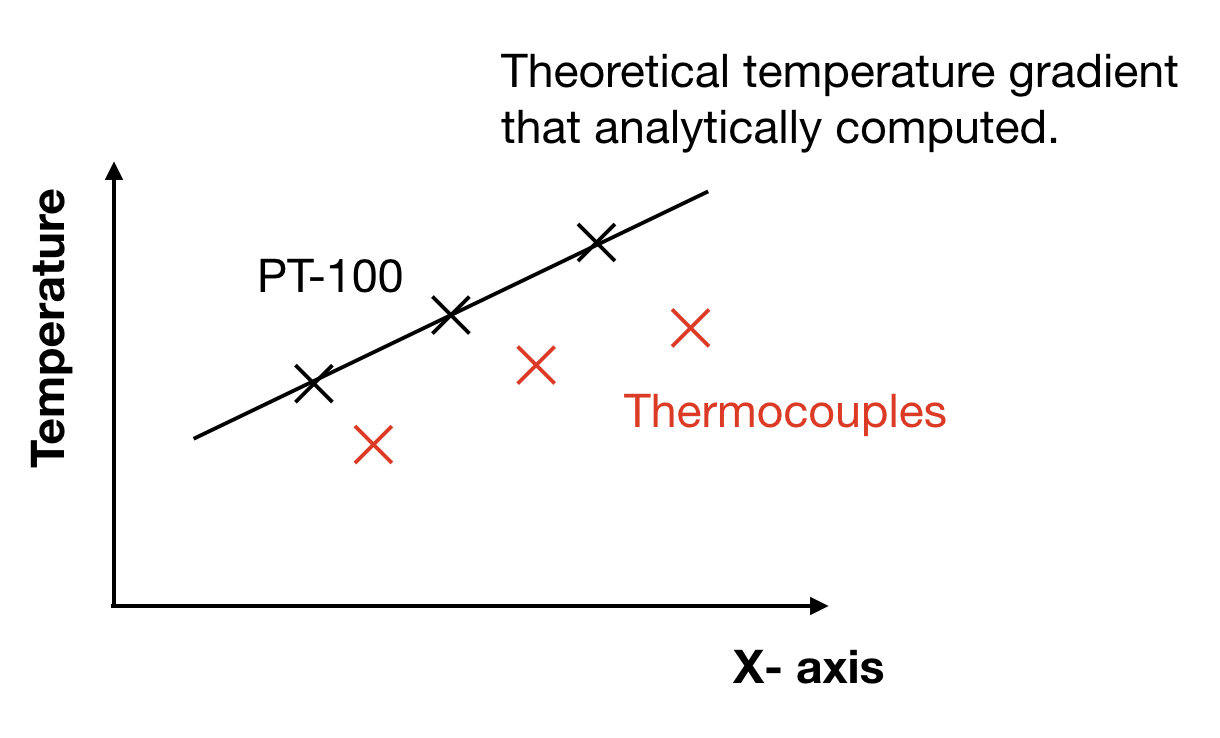
\includegraphics[width=0.47\textwidth,natwidth=750,natheight=300]{fig/thermocouple_calibration.png}
  \caption{Thermocouples are always located under PT-100 before temperature calibration}
  \label{temperature_calibration}
  \vspace{0zh}
\end{figure}

\newpage
  \item Fully developed length\\
  In figure.2., the length of entrance part in the test-section is 1.2 [m].
  To check the length of fully developped flow vary with Reynolds number wheather if there is a limitation of
flow speed to do a experiment, or not.\\
  \item Three parameters (Nu, Re, Pr)\\
  Experimental data and correlations is compared.
  In a correlation, the Prandtl number is constant.
  However, experimental Prandtl number is not constant because the fluid properties vary with temperature.
  The aim is to set Prandlt number level and vary the Reynolds number.
  There are only two parameters can be descrived on figures.
  The only choice is to take average Prandlt number and plot Nusselt and Reynolds number.
  Figure.10 shows only two parameter which are available to plot 2-D figures.
\begin{figure}[h]
\vspace{-2zh}
  \centering
  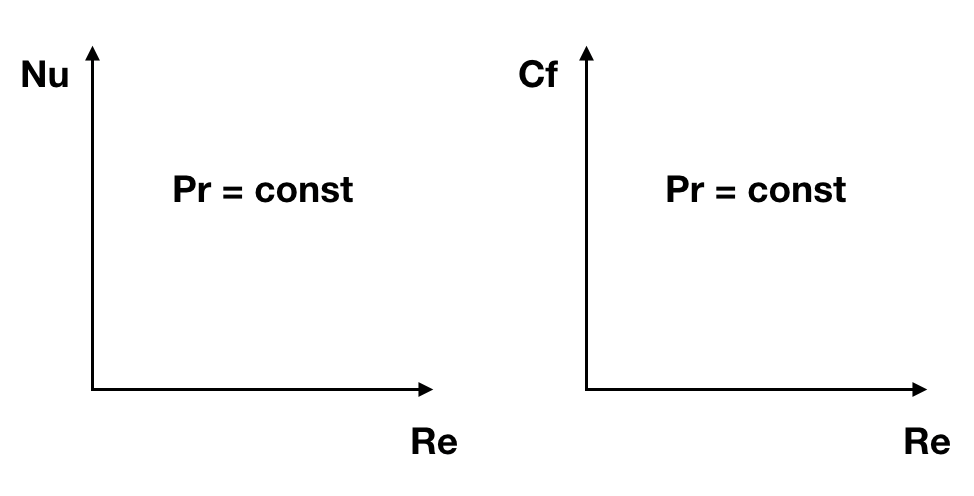
\includegraphics[width=0.47\textwidth,natwidth=750,natheight=300]{fig/three_parameters.png}
  \caption{Only two parameters ``Nu and Re'' and ``Cf and Re'' can be descrived in figures.}
  \label{three_parameters}
  \vspace{0zh}
\end{figure}

  \item The influence of enthaply, changing with pump power\\
  If we change pump power, not only flow speed but also heat transfer and enthaply change.
  For example, as increasing pump power, increasing flow speed and decreasing Prandtl number vary with heat transfer rate.
  Calcurating enthalpy, it would be easir to take Prandlt and Reynolds number which we wanted.
  Figure.11 shows many factors related in increasing pump.
\begin{figure}[htbp]
\vspace{3zh}
  \centering
  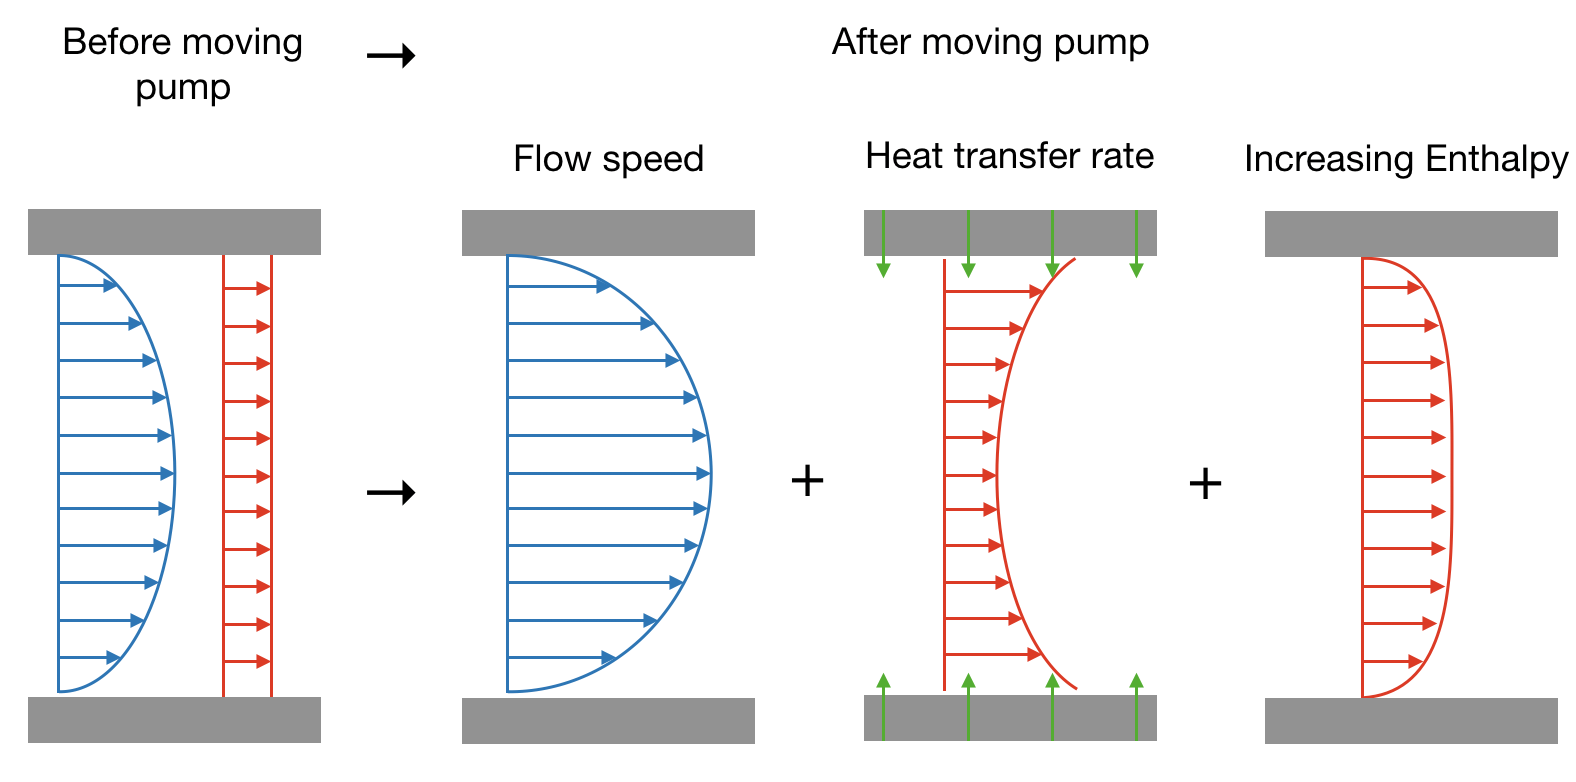
\includegraphics[width=0.47\textwidth,natwidth=750,natheight=300]{fig/pump_enthalpy.png}
  \caption{Changing pump speed, vary with flow speed, heat transfer rate and enthalpy.}
  \label{pump_enthalpy}
  \vspace{0zh}
\end{figure}
\newpage  
  \item Thermal contact resistant\\
  To avoid any influence of electronic current used for heating pipe, temperature sensors are electoronicaly isolated against stainless pipe in heated test-section.
  Calcurating any influence of thermal contact resistant between those two materials.\\
  \item Property of operating liquid dependence with long period of time\\
  It is unrealistic to change an operating liquid every experiments because it cost a lot and takes time.
  We need to use the same test liquid for long period of time.
  The fluid properties are taken at the bigining only one time.
  Fluid properties are really important issue in this research.
  Therefore, I want to search about lifuid properties dependence on time.\\
  \item Low temperature cooling\\
  In the heated part, the tube wall are heated electrically by welder.
  It is easy to make constant heat flux condition at high temperature.
  However, not so many ideas are available to maintain the 1[m] pipe low temperature.\\
  \item Appling turbulent intencity\\
  \item Appling Knudsen number\\
  \item Gnienski correlation\\
  Gnienski showed transitional flow as a liner interpolation between turbulent and laminar flow.
  Propose in case of non-liner correspond.
%  \item Temperature genelation(round?)\\
%  \item Corrilation between enthalpy and temperature profile
%  \item Outside temperature unceirtenty
%  \item Pipe surface roughness
\end{enumerate}

%Many studies have pointed out that heat transfer coefficient vary depending on the type of flow: laminar, transition and turbulent.
%Gnienlinski\cite{Gnienlinski2010} showed calculation method for laminar heat transfer coefficient of two kinds of boundary conditions. (I) Constant wall temperature (UWT) and (I\hspace{-.1em}I) Constant heat flux (UHF).
%
%\begin{equation}
%Nu_{lam}=\sqrt[3]{Nu_{1}^{3}+b^{3}+(Nu_{2}-b)^{3}+Nu_{3}^{3}}\label{Nu_laminar}
%\end{equation}
%For a cylindical pipe flow, the factor b is equal to b=3.
%\\For fully developed thermal and hydrodynamic flow the heat transfer coeficient.
%Graetz number define as Gz.
%\begin{equation}
%Nu_{1}=3.66
%\end{equation}
%\begin{equation}
%Nu_{2}=1.615\cdot \sqrt[3]{Gz}
%\end{equation}
%\begin{equation}
%Nu_{3}=\sqrt[6]{\frac{2}{1+22\cdot Pr}}\cdot Gz
%\end{equation}
%For a constant heat flux (UHF) over the heat transfer surface, those equations take the effect of the thermal boundary condition at heat transfering surface into account.
%\begin{equation}
%Nu_{1}=4.364
%\end{equation}
%\begin{equation}
%Nu_{2}=1.953\cdot \sqrt[3]{Gz}
%\end{equation}
%\begin{equation}
%Nu_{3}=0.924\cdot Pr^{\frac{1}{3}}\cdot \sqrt{Re\cdot \frac{d_{h}}{l}}
%\end{equation}
%Petukhvov and Kirillov\cite{Petukhov1958} showed calculation method for turbulent flow.
%\begin{equation}
%Nu_{turb}=\frac{\frac{\xi}{8}\cdot Re\cdot Pr}{(1+12.7\cdot \frac{\xi}{8})^{0.5}\cdot (Pr^{\frac{2}{3}}-1)}\cdot(1+(\frac{d_{h}}{l})^{\frac{2}{3}})\label{Nu_turblent}
%\end{equation}
%\begin{equation}
%\xi=(1.8\log{10}Re-1.5)^{-2}
%\label{Nu_turblent_xi}
%\end{equation}


%Bertsche et al,\cite{Bertsche2016} focused on reliable prediction of heat transfer coefficient for transitional flows.
%In their study, Bertsche et al, showed experimental heat transfer coefficients for Reynolds number $500 < Re < 23000$ and Prandtl number $7 < Pr < 41$.

%\section*{Acknowledgment}
%I would like to thank my thesis advisors Prof. Helfried Steiner and Prof. Guenter Brenn of the Institute of Fluid Mechanics and Heat Transfer at Graz University of Technology.
%%The door to Prof. Shirai of Mechanical Engineering department at Shibaura Institute of Technology was always support my studying abroad.
%I am also grateful to Dr. Shirai of Mechanical Engineering department at Shibaura Institute of Technology.
%I am extremely thankful and indebted to him for sharing his experiments.
%I would also like to thank Dr. Tange allowed my studying in Graz, Austria.


\begin{thebibliography}{00}
 \bibitem{Frank} Frank P. Incropera, David P. DeWitt, ``Fundamentals of Heat and Mass Transfer,'' 4th edition., WILEY, 1996.
 \bibitem{Gnienlinski2010} V. Gnienlinski, ``Heat Transfer in Laminar Flow,'' VDI Heat Atlas, second ed., Springer Verlag, 2010 (Chapter Ga 1-7), Section 3.
 \bibitem{Petukhov1958} B.S. Petukhov, V.V. kirillov, Teploenergetika 4 (1958) 91-98.
 \bibitem{Bertsche2016} Dirk Bertsche, Paul Knipper, Thomas Wetzel, ``Experimental investigation on heat transfer in laminar, transitional and turbulent circular pipe flow,'' International Journal of Heat Transfer, 95 (2016) 1008-1018.
\bibitem{Christphan2018} Christphan, ``Title of paper if known,'' unpublished, 2018.
\bibitem{Konakov1954} Konakov, ``Eine neue Formel fr den Reibungskoezienten glatter Rohre,'' Bericht der Akademie der Wissenschaften der UDSSR 51.7, 503-506.
% \bibitem{b5} R. Nicole, ``Title of paper with only first word capitalized,'' J. Name Stand. Abbrev., in press.
% \bibitem{b6} Y. Yorozu, M. Hirano, K. Oka, and Y. Tagawa, ``Electron spectroscopy studies on magneto-optical media and plastic substrate interface,'' IEEE Transl. J. Magn. Japan, vol. 2, pp. 740--741, August 1987 [Digests 9th Annual Conf. Magnetics Japan, p. 301, 1982].
% \bibitem{b7} M. Young, The Technical Writer's Handbook. Mill Valley, CA: University Science, 1989.

%\bibliography{junsrt}
%\bibliography{project_forced_convective@Graz.bib}

\end{thebibliography}
%\vspace{12pt}
%\color{red}
%IEEE conference templates contain guidance text for composing and formatting conference papers. Please ensure that all template text is removed from your conference paper prior to submission to the conference. Failure to remove the template text from your paper may result in your paper not being published.

\end{document}
